% Copyright (C) 2017 - 2019 - Michael Baudin

  \documentclass{beamer}

%\setbeameroption{hide notes}
%\setbeameroption{show notes}
%\setbeameroption{show only notes}

  % Copyright (C) 2012 - 2013 - EDF R&D - Michael Baudin

\setbeameroption{hide notes}
%\setbeameroption{show notes}
%\setbeameroption{show only notes}
%\mode<presentation>{\usetheme{EDF09}}

% Configuration beamer
\usetheme{Montpellier}
\setbeamertemplate{navigation symbols}{} % Remove navigation
\useoutertheme{infolines}
\setbeamertemplate{theorems}[numbered] 
% Utilise des fonts serif, pour �viter les pb de fonte
\usefonttheme{serif} 
\setbeamertemplate{caption}[numbered]


\usepackage[utf8]{inputenc}
\usepackage[T1]{fontenc}


\usepackage[french]{babel}
\uselanguage{French}
\languagepath{French}

% Scilab macros
\newcommand{\sciobj}[1]{\texttt{#1}}
\newcommand{\scifile}[1]{\texttt{#1}}

% Python macros
\newcommand{\pyobj}[1]{\textcolor{blue}{\texttt{#1}}}

\def\RR{\mathbb{R}}
\def\NN{\mathbb{N}}
\def\ZZ{\mathbb{Z}}
\def\bx{{\bf x}}

% To highlight source code
\usepackage{listingsutf8}
\lstset{inputencoding=utf8/latin1}

\definecolor{darkgreen}{rgb}{0,0.5,0}
\definecolor{violet}{rgb}{0.5,0,1}
\lstset{
  % general command to set parameter(s)
   basicstyle=\scriptsize\ttfamily, %
   keywordstyle=\color{violet}\bfseries,%
   commentstyle=\color{darkgreen}\bfseries,%
   showspaces=false,%
   stringstyle=\color{red}\bfseries
}

\hypersetup{
    %bookmarks=true,         % show bookmarks bar?
    %unicode=false,          % non-Latin characters in Acrobat�s bookmarks
    %pdftoolbar=true,        % show Acrobat�s toolbar?
    %pdfmenubar=true,        % show Acrobat�s menu?
    %pdffitwindow=false,     % window fit to page when opened
    %pdfstartview={FitH},    % fits the width of the page to the window
    %pdftitle={My title},    % title
    %pdfauthor={Author},     % author
    %pdfsubject={Subject},   % subject of the document
    %pdfcreator={Creator},   % creator of the document
    %pdfproducer={Producer}, % producer of the document
    %pdfkeywords={keyword1} {key2} {key3}, % list of keywords
    %pdfnewwindow=true,      % links in new window
    colorlinks=true,       % false: boxed links; true: colored links
    %linkcolor=red,          % color of internal links (change box color with linkbordercolor)
    %citecolor=green,        % color of links to bibliography
    %filecolor=magenta,      % color of file links
    urlcolor=blue           % color of external links
}

\title[OpenTURNS]{OpenTURNS and its graphical interface}

\author[Baudin et al.]{
Micha�l Baudin \inst{1} \and
Anne Dutfoy \inst{1} \and
Anthony Geay \inst{1} \and
Anne-Laure Popelin \inst{1} \and
Aur�lie Ladier \inst{2} \and
Julien Schueller \inst{2} \and
Thierry Yalamas \inst{2}
}

\institute[EDF-Phim�ca]{
\inst{1} EDF R\&D. 6, quai Watier, 78401, Chatou Cedex - France, michael.baudin@edf.fr \and %
\inst{2} Phimeca Engineering. 18/20 boulevard de Reuilly, 75012 Paris - France, yalamas@phimeca.com
}

\date[]{15 June 2017, UNCECOMP 2019, Rhodes, Greece}

%%%%%%%%%%%%%%%%%%%%%%%%%%%%%%%%%%%%%%%%%%%%%%%%%%%%%%%%%%%%%%%%%%%%%%%%%%%%%

  \begin{document}

%%%%%%%%%%%%%%%%%%%%%%%%%%%%%%%%%%%%%%%%%%%%%%%%%%%%%%%%%%%%%%%%%%%%%%%%%%%%%

  \begin{frame}
  \titlepage
  
  \begin{columns}
    \column{0.45\textwidth}
  \begin{center}

\includegraphics[height=0.15\textheight]{figures/edf.jpg}
\end{center}
    \column{0.1\textwidth}
	
    \column{0.45\textwidth}
  \begin{center}

\includegraphics[height=0.15\textheight]{figures/logo_phimeca.png}
\end{center}
  \end{columns}

  \end{frame}

%%%%%%%%%%%%%%%%%%%%%%%%%%%%%%%%%%%%%%%%%%%%%%%%%%%%%%%%%%%%%%%%%%%%%%%%%%%%%

\begin{frame}
\frametitle{Contents}
\tableofcontents
\end{frame}

%%%%%%%%%%%%%%%%%%%%%%%%%%%%%%%%%%%%%%%%%%%%%%%%%%%%%%%%%%%%%%%%%%%%%%%%%%%%%
\section{Introduction}

%%%%%%%%%%%%%%%%%%%%%%%%%%%%%%%%%%%%%%%%%%%%%%%%%%%%%%%%%%%%%%%%%%%%%%%%%%%%%

\begin{frame}
\frametitle{OpenTURNS: \url{www.openturns.org}}


    \begin{center}
    
\includegraphics[width=0.8\textwidth]{figures/OT.pdf}
    \end{center}
	
\begin{itemize}
\item Multivariate probabilistic modeling including dependence
\item Numerical tools dedicated to the treatment of uncertainties
\item Generic coupling to any type of physical model
\item Open source, LGPL licensed, C++/Python library
\end{itemize}


\end{frame}

\note{
OpenTURNS is a software for uncertainty quantification, uncertainty propagation, 
sensitivity analysis and metamodeling. 

It is developped by five parterns : EDF, Phim�ca, Airbus, IMACS and ONERA.

The software is available with the open source LGPL licence on Linux and Windows. 


In order to use OpenTURNS, you can use directly the C++ library, or 
program your Python scripts. 
}
%%%%%%%%%%%%%%%%%%%%%%%%%%%%%%%%%%%%%%%%%%%%%%%%%%%%%%%%%%%%%%%%%%%%%%%%%%%%%

\begin{frame}
\frametitle{OpenTURNS: \url{www.openturns.org}}

\begin{center}
   \begin{tabular}{ccccc}
   
\includegraphics[width=0.07\textwidth]{figures/logoEDF_Anne.png}&
   
\includegraphics[width=0.12\textwidth]{figures/LogoAirbus.png}&
   
\includegraphics[width=0.12\textwidth]{figures/logo_phimeca.png}&
   
\includegraphics[width=0.12\textwidth]{figures/logo_Imacs.png}
   
\includegraphics[width=0.30\textwidth]{figures/logo_ONERA.jpg}&
   \end{tabular}
\end{center}

\vspace*{0.05cm}
\begin{itemize}
\item Linux, Windows
\item First release : 2007
\item 4 full time developers
\item Users $\approx 1000$, mainly in France
(10900 Conda downloads in 2016-2017)
\item Project size (2018) : 720 classes, more than 6000 services
\end{itemize}

\end{frame}

%%%%%%%%%%%%%%%%%%%%%%%%%%%%%%%%%%%%%%%%%%%%%%%%%%%%%%%%%%%%%%%%%%%%%%%%%%%%%

\begin{frame}[containsverbatim]
\frametitle{OpenTURNS: content}

    \begin{center}
    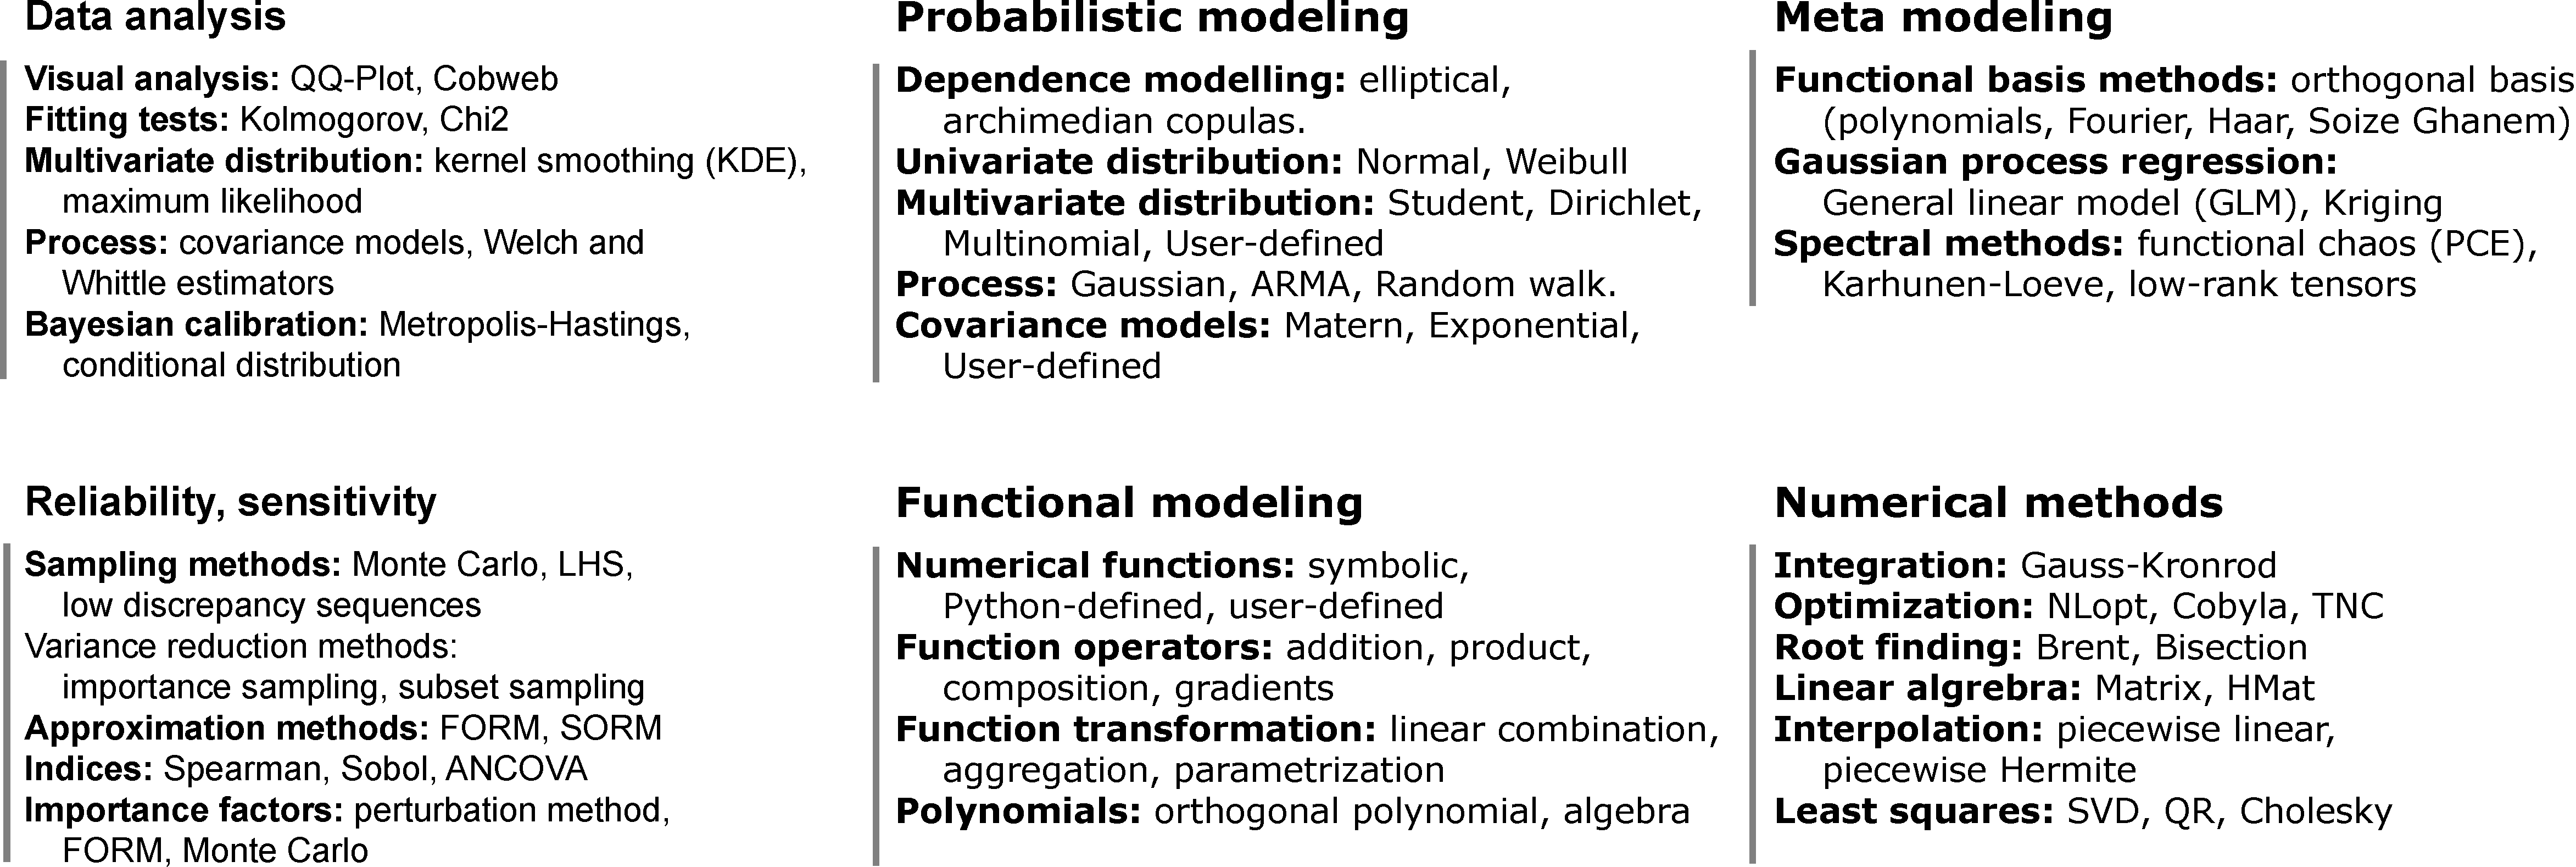
\includegraphics[width=\textwidth]{figures/OpenTURNS-Content-Table.pdf}
    \end{center}

   \begin{tabular}{@{}c@{}c@{}c@{}c@{}c@{}}
   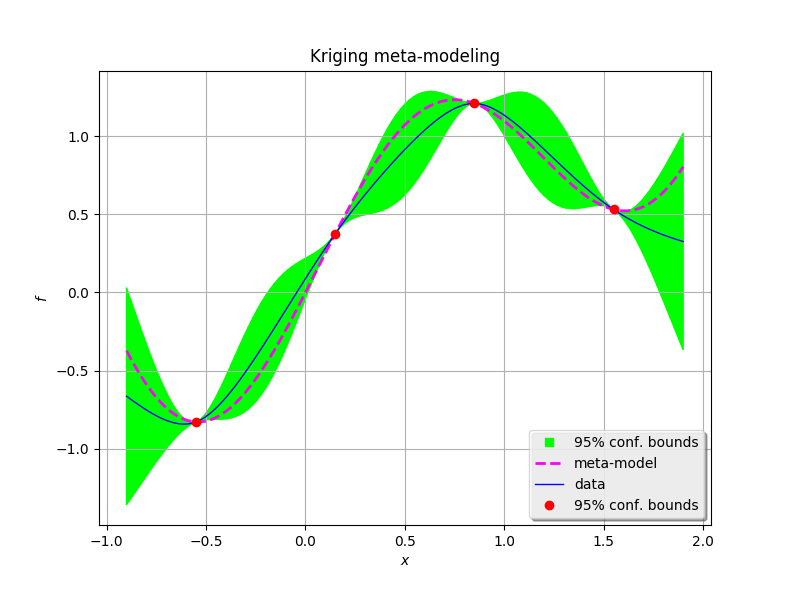
\includegraphics[width=0.2\textwidth]{figures/plot_kriging.png}&
   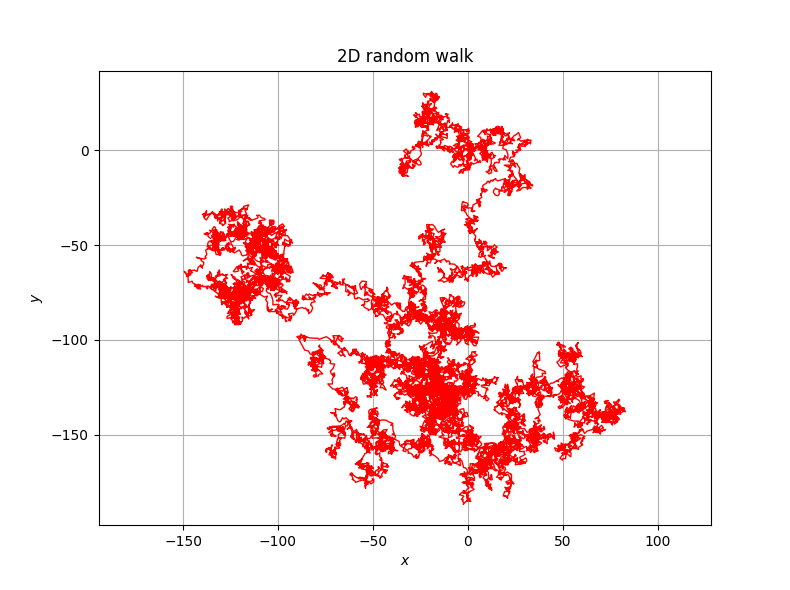
\includegraphics[width=0.2\textwidth]{figures/plot_random_walk.png}&
   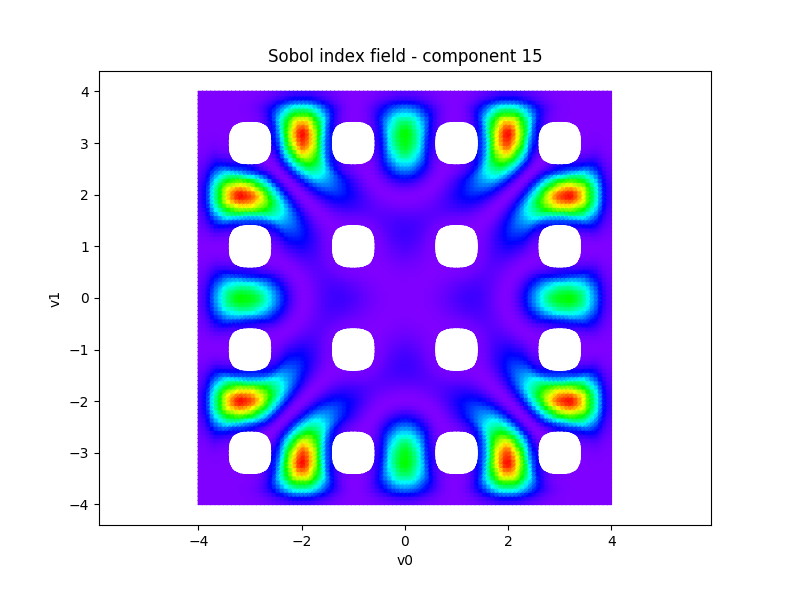
\includegraphics[width=0.2\textwidth]{figures/plot_sobol_field.png}&
   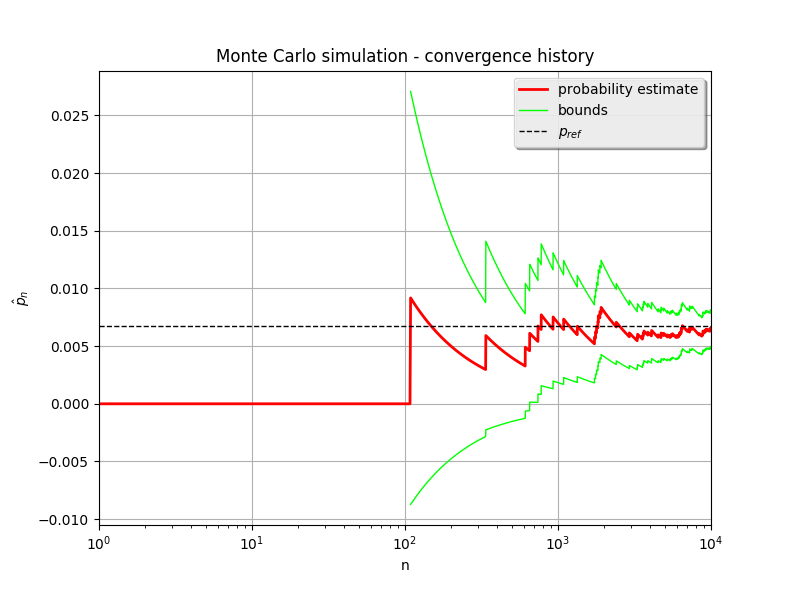
\includegraphics[width=0.2\textwidth]{figures/plot_monte_carlo.png}&
   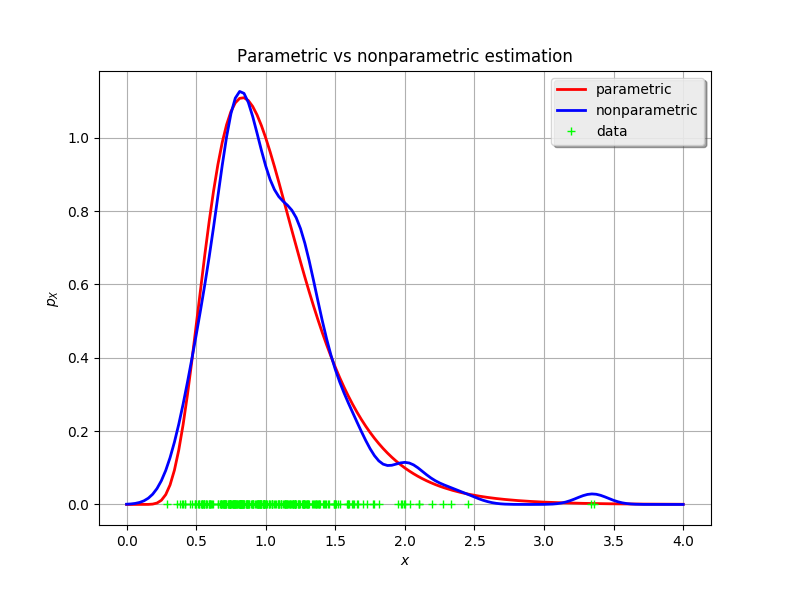
\includegraphics[width=0.2\textwidth]{figures/plot_distribution_fitting.png}
   \end{tabular}
\end{frame}


%%%%%%%%%%%%%%%%%%%%%%%%%%%%%%%%%%%%%%%%%%%%%%%%%%%%%%%%%%%%%%%%%%%%%%%%%%%%%

\begin{frame}[containsverbatim]
\frametitle{OpenTURNS: documentation}

\small{

\begin{columns}
    \column{0.5\textwidth}

    \begin{center}
    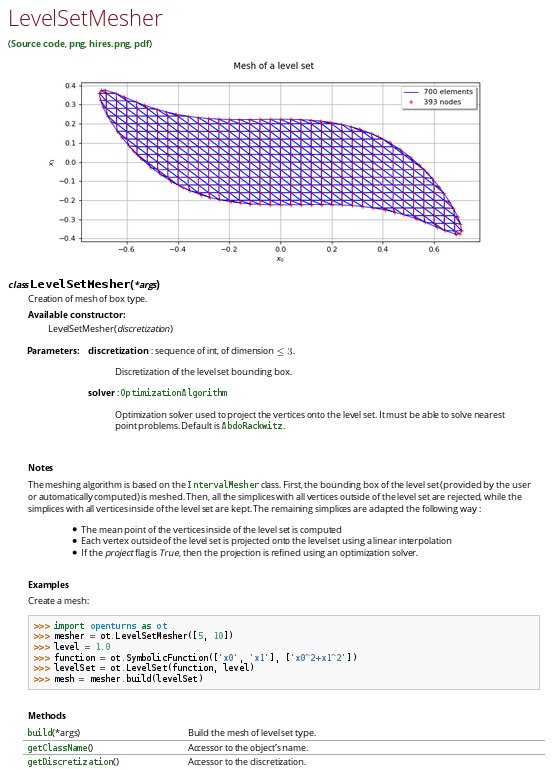
\includegraphics[width=0.8\textwidth]{figures/exClasses.png}
    \end{center}

    \column{0.5\textwidth}

    \begin{center}
    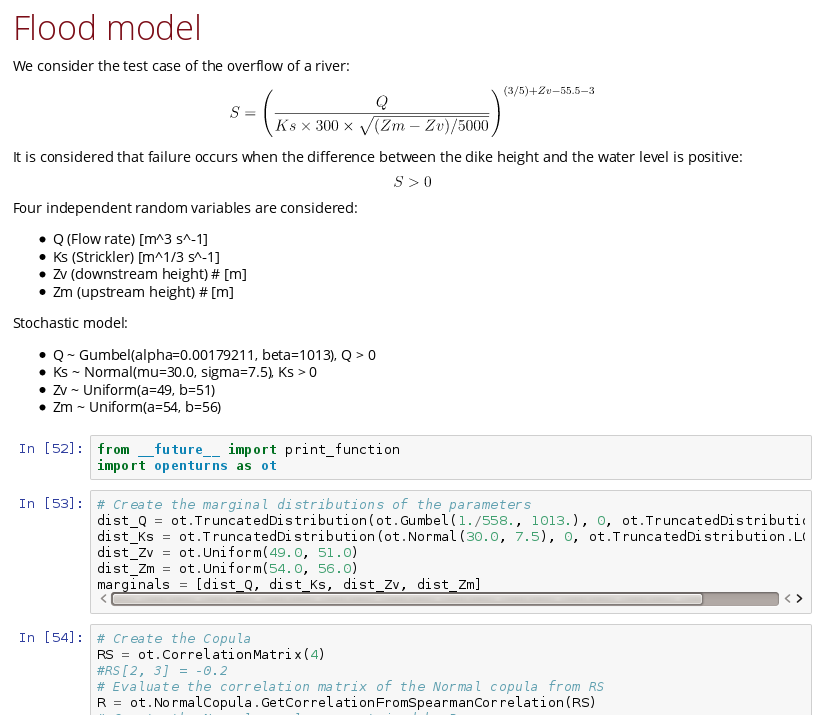
\includegraphics[width=0.9\textwidth]{figures/exRefGuide.png}
    \end{center}
	
\end{columns}

}
\end{frame}

% %%%%%%%%%%%%%%%%%%%%%%%%%%%%%%%%%%%%%%%%%%%%%%%%%%%%%%%%%%%%%%%%%%%%%%%%%%%%%

\section{Example of incremental algorithms}


% %%%%%%%%%%%%%%%%%%%%%%%%%%%%%%%%%%%%%%%%%%%%%%%%%%%%%%%%%%%%%%%%%%%%%%%%%%%%%

\begin{frame}[containsverbatim]
\frametitle{OpenTURNS: estimate the mean}

See the Jupyter Notebook.

\scriptsize{

\lstset{language=python}
\begin{lstlisting}
from openturns.viewer import View
import openturns as ot
from math import sqrt

ot.RandomGenerator.SetSeed(0)

# 1. The function G
def functionCrue(X) :
    Q, Ks, Zv, Zm = X
    alpha = (Zm - Zv)/5.0e3
    H = (Q/(Ks*300.0*sqrt(alpha)))**(3.0/5.0)
    S = [H + Zv - (55.5 + 3.0)]
    return S

# Creation of the problem function
g = ot.PythonFunction(4, 1, functionCrue) 
g = ot.MemoizeFunction(g)
\end{lstlisting}

}

\end{frame}

% %%%%%%%%%%%%%%%%%%%%%%%%%%%%%%%%%%%%%%%%%%%%%%%%%%%%%%%%%%%%%%%%%%%%%%%%%%%%%

\begin{frame}[containsverbatim]
\frametitle{OpenTURNS: estimate the mean}

\begin{columns}
    \column{0.65\textwidth}

\scriptsize{

\lstset{language=python}
\begin{lstlisting}
# 2. Random vector definition
myParamQ = ot.GumbelAB(1013., 558.)
Q = ot.ParametrizedDistribution(myParamQ)
otLOW = ot.TruncatedDistribution.LOWER
Q = ot.TruncatedDistribution(Q, 0, otLOW)
Ks = ot.Normal(30.0, 7.5)
Ks = ot.TruncatedDistribution(Ks, 0, otLOW)
Zv = ot.Uniform(49.0, 51.0)
Zm = ot.Uniform(54.0, 56.0)

# 3. View the PDF
Q.setDescription(["Q (m3/s)"])
View(Q.drawPDF()).show()
\end{lstlisting}

}

\column{0.35\textwidth}
	\begin{center}
	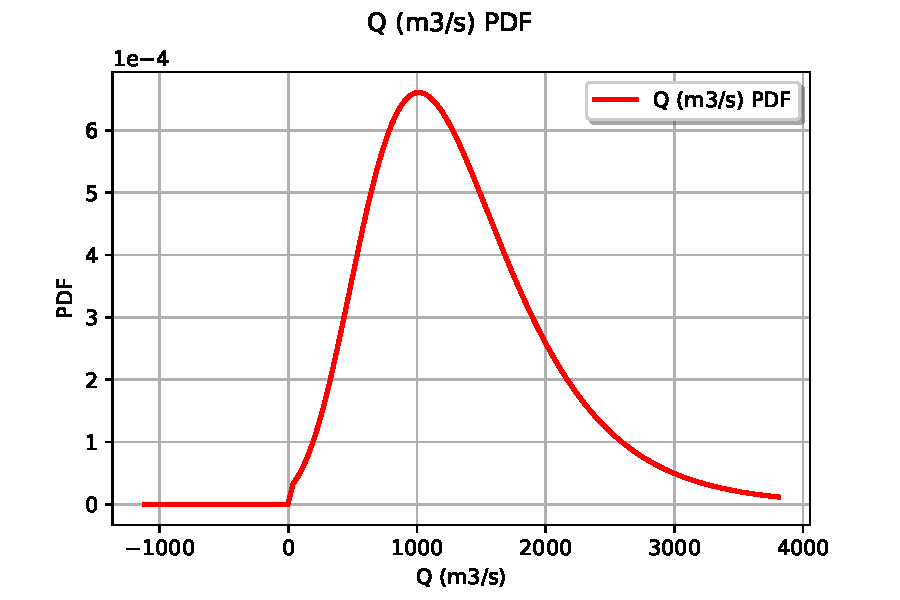
\includegraphics[width=0.95\textwidth]{figures/Q.pdf}
	\end{center}


\end{columns}

\end{frame}

% %%%%%%%%%%%%%%%%%%%%%%%%%%%%%%%%%%%%%%%%%%%%%%%%%%%%%%%%%%%%%%%%%%%%%%%%%%%%%

\begin{frame}[containsverbatim]
\frametitle{OpenTURNS: estimate the mean}

\begin{columns}
    \column{0.65\textwidth}

\scriptsize{

\lstset{language=python}
\begin{lstlisting}
# 4. Create the joint distribution function, 
#    the output and the event. 
X = ot.ComposedDistribution([Q, Ks, Zv, Zm])
Y = ot.RandomVector(g, ot.RandomVector(X))

# 5. Estimate expectation with simple Monte-Carlo
sampleSize = 10000
sampleX = X.getSample(sampleSize)
sampleY = g(sampleX)
sampleMean = sampleY.computeMean()
print("Mean=%f" % (sampleMean[0]))
\end{lstlisting}

Output: 
\begin{lstlisting}
Mean by MC =-5.937845
\end{lstlisting}

}

\column{0.35\textwidth}

\end{columns}

\end{frame}
% %%%%%%%%%%%%%%%%%%%%%%%%%%%%%%%%%%%%%%%%%%%%%%%%%%%%%%%%%%%%%%%%%%%%%%%%%%%%%

\begin{frame}[containsverbatim]
\frametitle{OpenTURNS: estimate the mean}

\begin{columns}
    \column{0.65\textwidth}

\scriptsize{

\lstset{language=python}
\begin{lstlisting}
# 6. Estimate expectation with algorithm
algo = ot.ExpectationSimulationAlgorithm(Y)
algo.setMaximumOuterSampling(1000)
algo.setBlockSize(1)
algo.setCoefficientOfVariationCriterionType('NONE')
algo.run()
result = algo.getResult()
expectation = result.getExpectationEstimate()
print("Mean by ESA = %f " % expectation[0])
expectationDistribution = result.getExpectationDistribution()
View(expectationDistribution.drawPDF())
\end{lstlisting}

Output: 
\begin{lstlisting}
Mean by ESA = -5.972516 
\end{lstlisting}

}

\column{0.35\textwidth}

	\begin{center}
	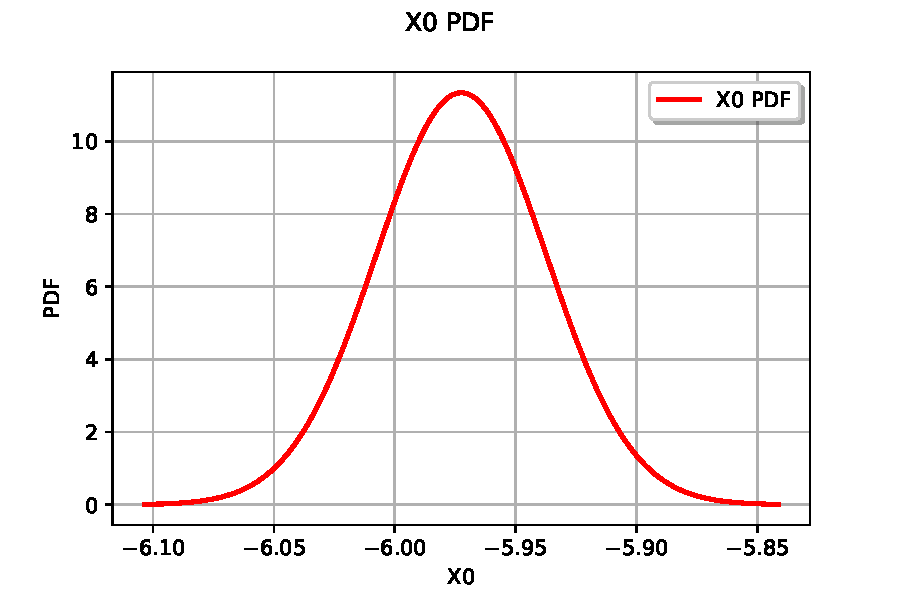
\includegraphics[width=0.95\textwidth]{figures/MeanDistribution.pdf}
	\end{center}

\end{columns}

\end{frame}
%%%%%%%%%%%%%%%%%%%%%%%%%%%%%%%%%%%%%%%%%%%%%%%%%%%%%%%%%%%%%%%%%%%%%%%%%%%%%

\begin{frame}
\frametitle{SALOME}

  \begin{columns}
    \column{0.5\textwidth}
	
\begin{itemize}
\item Integration platform for pre and post processing, and 2D/3D numerical simulation 
\item Features : geometry, mesh, distributed computing
\item Visualization, data assimilation, uncertainty treatment
\item Partners : EDF, CEA, Open Cascade
\item Licence : LGPL
\item Linux, Windows
\item \url{www.salome-platform.org}
\end{itemize}

    \column{0.5\textwidth}

	\begin{center}
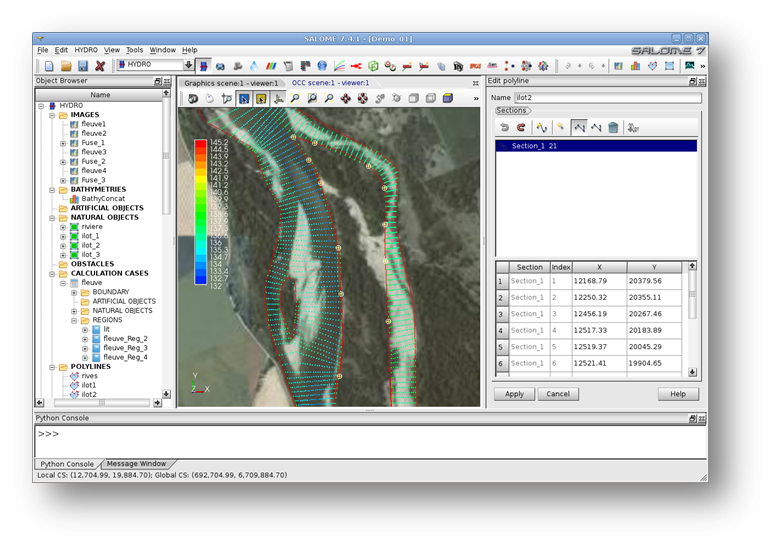
\includegraphics[width=0.95\textwidth]{figures/Salome-hydro-platform}
\end{center}

	\end{columns}
\end{frame}

%%%%%%%%%%%%%%%%%%%%%%%%%%%%%%%%%%%%%%%%%%%%%%%%%%%%%%%%%%%%%%%%%%%%%%%%%%%%%

\begin{frame}
\frametitle{The graphical user interface of \ot{}}
	
\begin{itemize}
\item Main goal : provide a graphical interface of 
\ot{} in SALOME
\item Features
	\begin{itemize}
	\item Uncertainty quantification (distribution fitting), 
	central tendency, sensitivity analysis, probability estimate, 
	meta-modeling
	\item Generic (not dedicated to a specific application)
	\item GUI language : English, French
	\end{itemize}

\item Partners : EDF, Phim�ca
\item Licence : LGPL

\item Schedule : 
	\begin{itemize}
	\item Since summer 2016, one EDF release per year
	\item On the internet : 2018
	\end{itemize}

\end{itemize}

\end{frame}

%%%%%%%%%%%%%%%%%%%%%%%%%%%%%%%%%%%%%%%%%%%%%%%%%%%%%%%%%%%%%%%%%%%%%%%%%%%%%

\section{Demo}

\begin{frame}
\frametitle{GUI : the demo}

\begin{center}
Demo time.
\end{center}

\end{frame}

%%%%%%%%%%%%%%%%%%%%%%%%%%%%%%%%%%%%%%%%%%%%%%%%%%%%%%%%%%%%%%%%%%%%%%%%%%%%%


\begin{frame}
\frametitle{GUI : outline}

\begin{itemize}
\item From scratch : 3 inputs, 2 outputs, sum, central dispersion study with default parameters
\item Open axialStressedBeam-python.xml : central dispersion with sample size 1000, Threshold P(G<0) with CV=0.05
\item Import crue-4vars-analytique.py : S.A. with sample size 1000, sort by size
\end{itemize}

\end{frame}


%%%%%%%%%%%%%%%%%%%%%%%%%%%%%%%%%%%%%%%%%%%%%%%%%%%%%%%%%%%%%%%%%%%%%%%%%%%%%
\section{Background}

\begin{frame}
\frametitle{UQ, the easy way}

Main goal : make UQ easy to use
\begin{itemize}
\item classical user-friendly algorithms with a 
state-of-the-art implementation,
\item default parameters of the algorithms whenever possible,
\item an easy access to the HPC resources,
\item an automated connection to the computer code.
\end{itemize}

Produce standard results :
\begin{itemize}
\item numerical results e.g. tables,
\item classical graphics.
\end{itemize}

\end{frame}

%%%%%%%%%%%%%%%%%%%%%%%%%%%%%%%%%%%%%%%%%%%%%%%%%%%%%%%%%%%%%%%%%%%%%%%%%%%%%

\begin{frame}
\frametitle{Overview (1/2)}

Inputs from the user :
\begin{itemize}
\item Physical model : symbolic, Python code or SALOME component
\item Probabilistic model : joint probability distribution function of the input.
\end{itemize}

Then :
\begin{itemize}
\item Central dispersion: estimates the central dispersion of the output Y (e.g. mean).
\item Threshold probability: estimates the probability that the output exceeds a given
threshold S.
\item Sensitivity analysis: estimates the importance of the inputs to the variability of the output.
\end{itemize}

\end{frame}

%%%%%%%%%%%%%%%%%%%%%%%%%%%%%%%%%%%%%%%%%%%%%%%%%%%%%%%%%%%%%%%%%%%%%%%%%%%%%

\begin{frame}
\frametitle{Overview (2/2)}

Probabilistic modeling :
\begin{itemize}
\item Distribution fitting from a sample
\item Dependence modeling (Gaussian copula)
\end{itemize}

Meta-modeling :
\begin{itemize}
\item Polynomial chaos (full or sparse)
\item Kriging
\end{itemize}

\end{frame}


%%%%%%%%%%%%%%%%%%%%%%%%%%%%%%%%%%%%%%%%%%%%%%%%%%%%%%%%%%%%%%%%%%%%%%%%%%%%%
\section{What's next ?}


\begin{frame}
\frametitle{Fields}
  \begin{columns}
    \column{0.5\textwidth}

Field example : 
\begin{itemize}
\item Input : 4 independent random variables
\item Output : height of the river Garonne on a 100 km segment
\item Computer code : TELEMAC2D
\item Quantity of interest : pointwise average over 70 000 random simulations
\end{itemize}

Roadmap : 
\begin{itemize}
\item Now : massive Python/\ot{} scripting
\item 2017-2018 : in the gui
\end{itemize}

    \column{0.5\textwidth}

\begin{center}
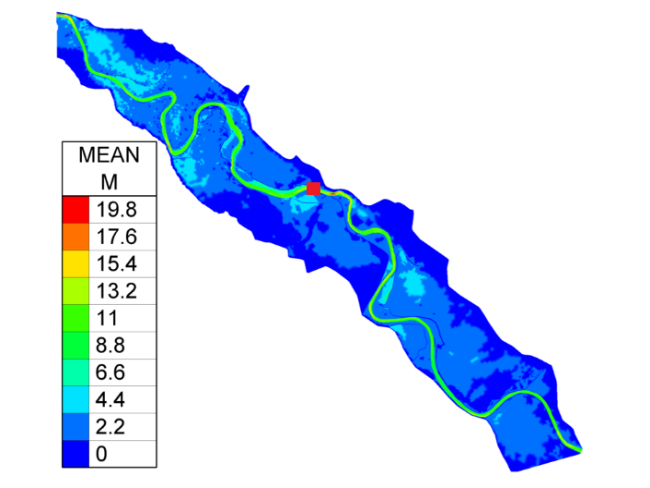
\includegraphics[height=0.5\textheight]{figures/image034.png}
\end{center}


	\end{columns}

\end{frame}

%%%%%%%%%%%%%%%%%%%%%%%%%%%%%%%%%%%%%%%%%%%%%%%%%%%%%%%%%%%%%%%%%%%%%%%%%%%%%

\begin{frame}
\frametitle{The end}

\begin{center}
Thanks !
\end{center}

\begin{center}
Questions ?
\end{center}

\end{frame}

%%%%%%%%%%%%%%%%%%%%%%%%%%%%%%%%%%%%%%%%%%%%%%%%%%%%%%%%%%%%%%%%%%%%%%%%%%%%%
\section{Extra slides}

\begin{frame}
\frametitle{Interactive uncertainty visualization with Paraview}

\begin{center}
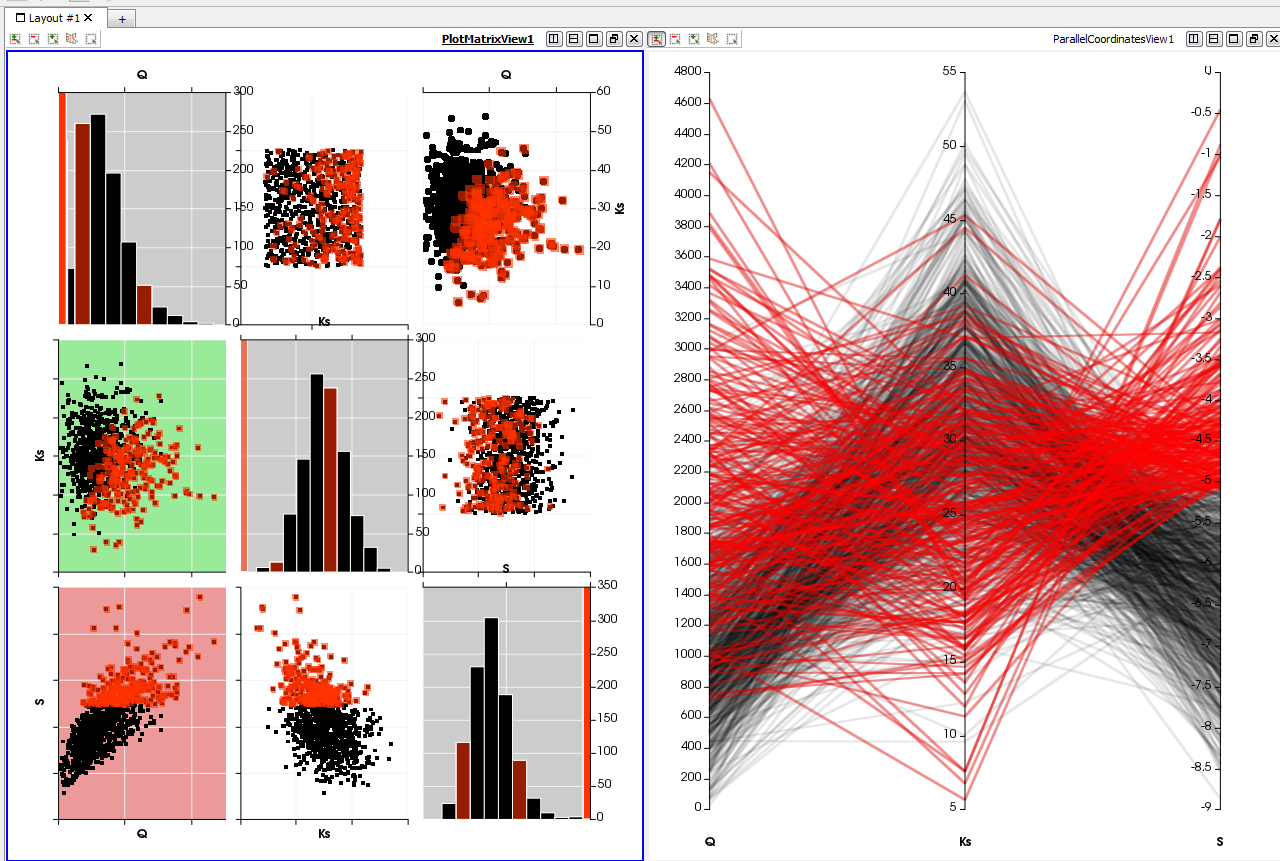
\includegraphics[width=0.9\textwidth]{figures/image032.png}
\end{center}

\end{frame}

%%%%%%%%%%%%%%%%%%%%%%%%%%%%%%%%%%%%%%%%%%%%%%%%%%%%%%%%%%%%%%%%%%%%%%%%%%%%%

\begin{frame}
\frametitle{Methodology}

\begin{center}
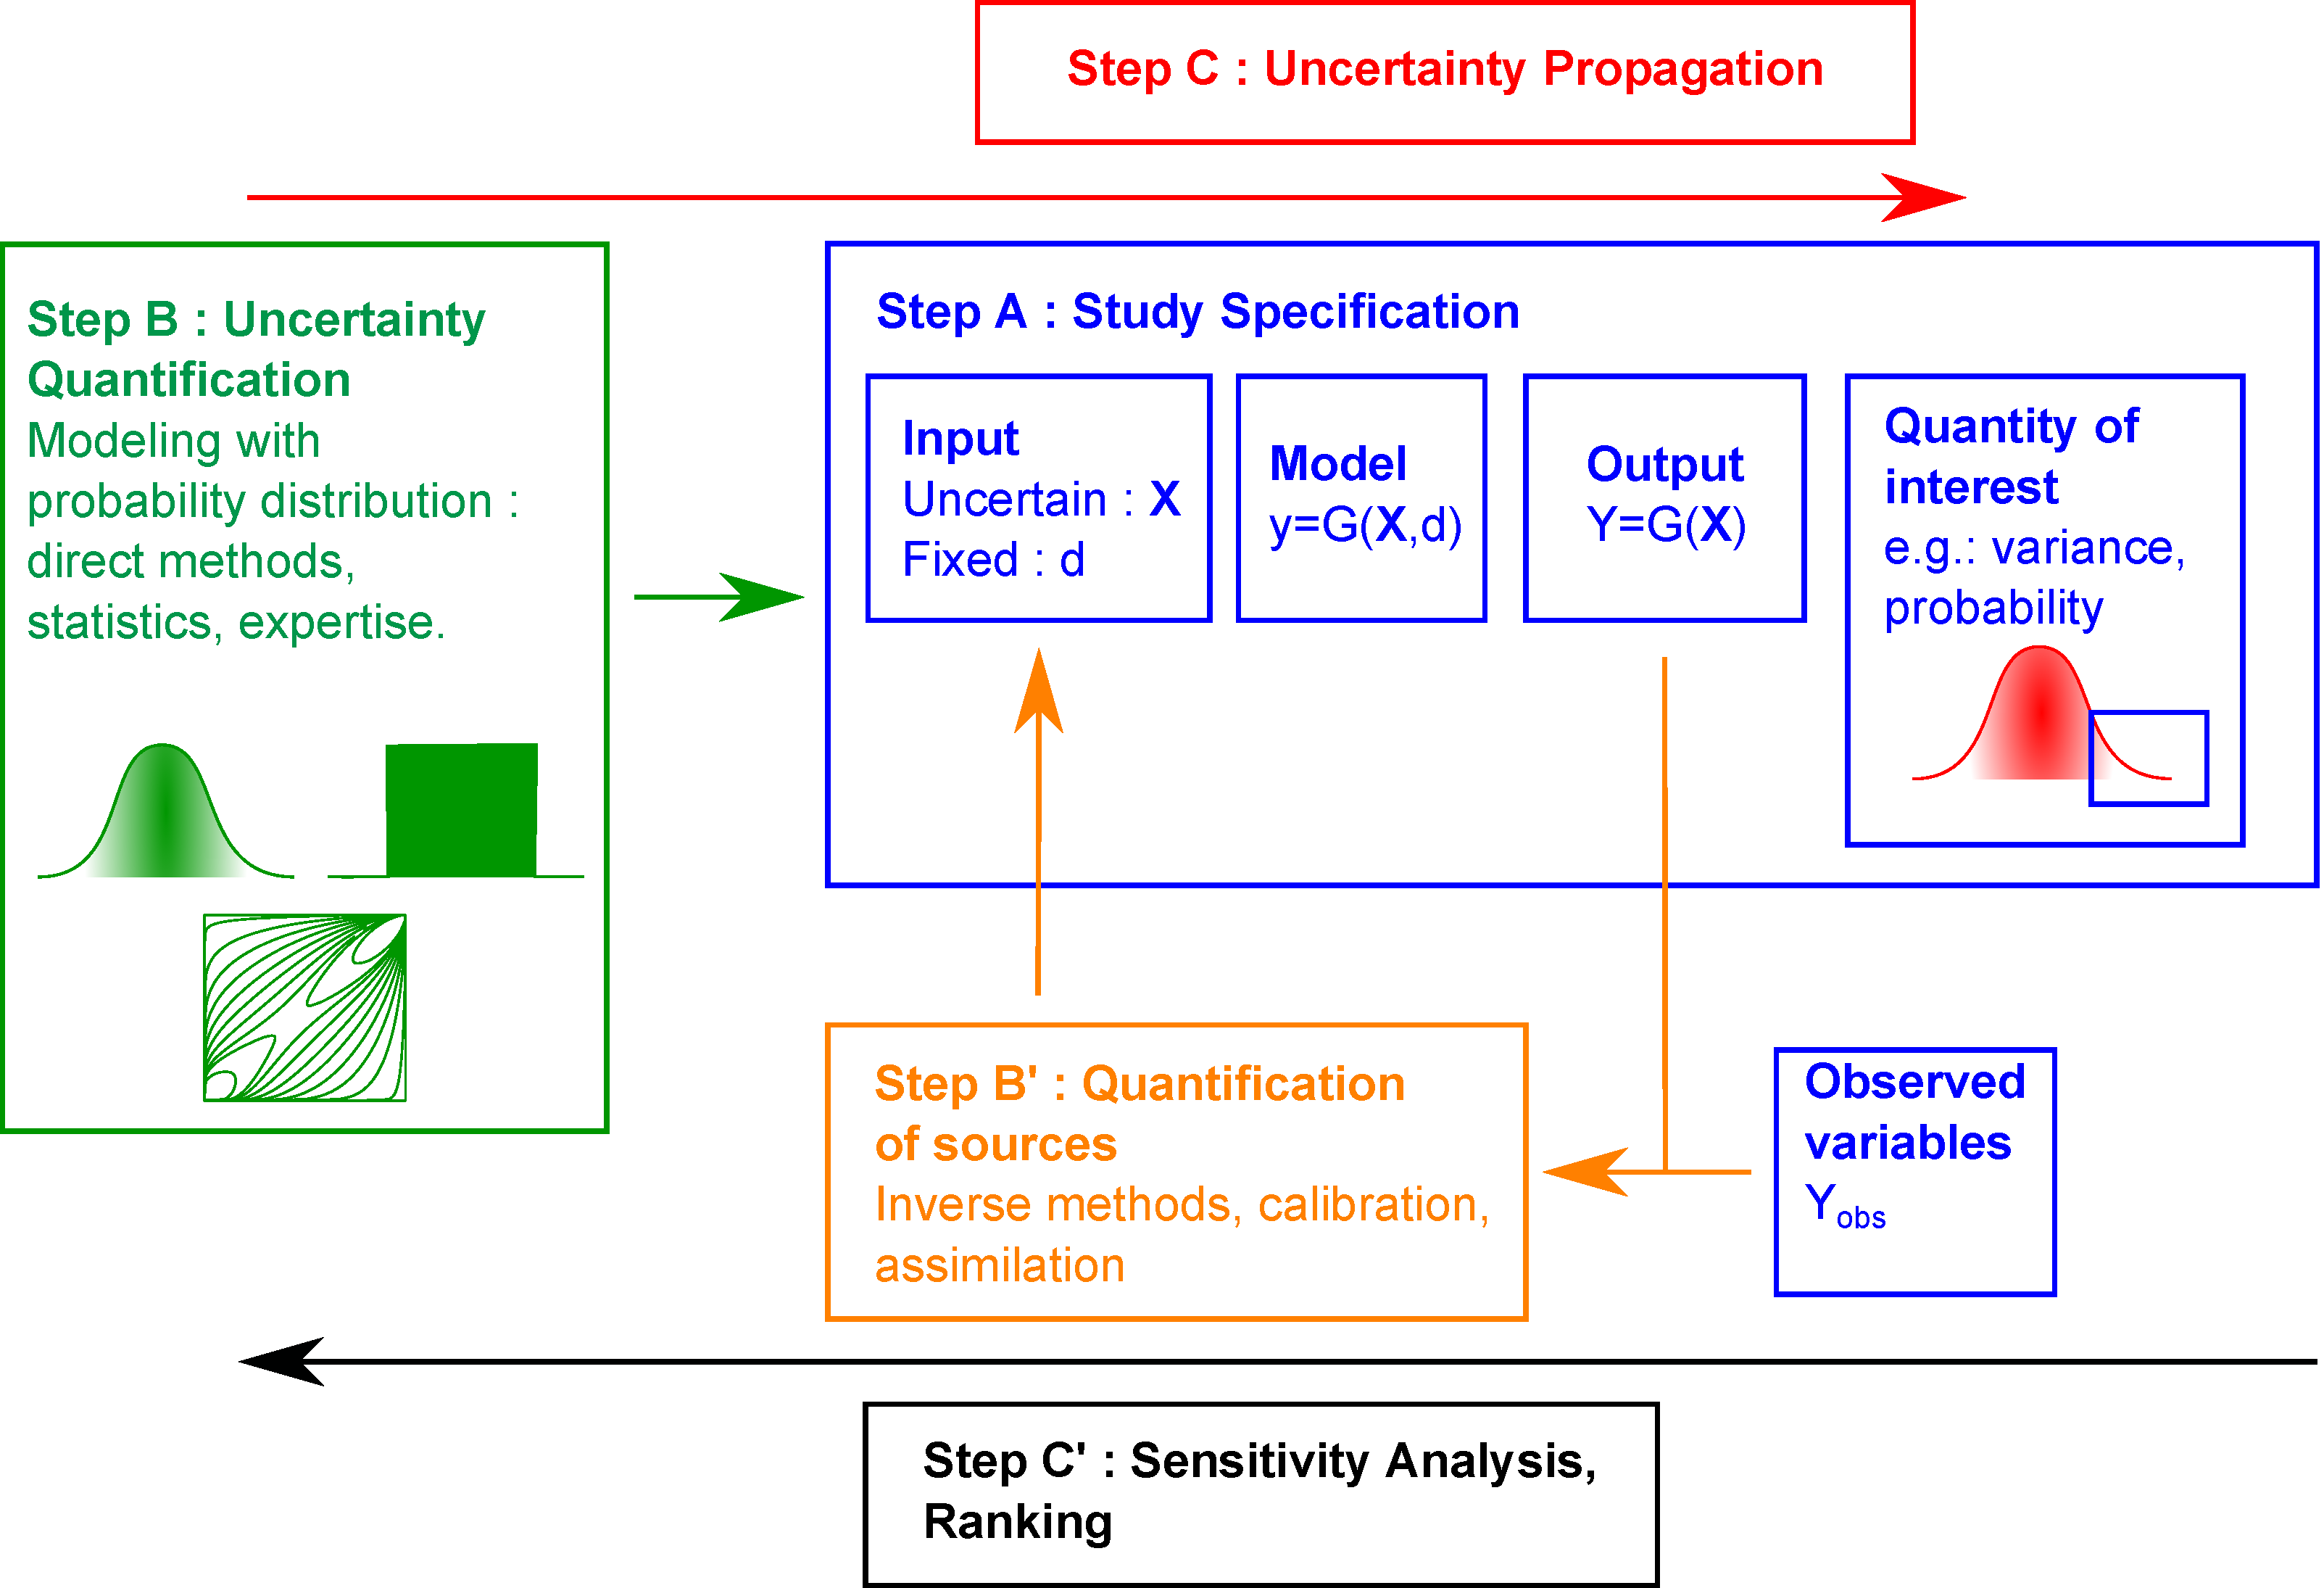
\includegraphics[width=0.9\textwidth]{figures/MethodologieIncertitude-EN.pdf}
\end{center}

\end{frame}

%%%%%%%%%%%%%%%%%%%%%%%%%%%%%%%%%%%%%%%%%%%%%%%%%%%%%%%%%%%%%%%%%%%%%%%%%%%%%

\begin{frame}
\frametitle{Software architecture}

  \begin{columns}
    \column{0.4\textwidth}
	
Two entry points:
\begin{itemize}
\item interactive,
\item Python.
\end{itemize}

Advantages of the Python programming of the GUI:
\begin{itemize}
\item unit tests,
\item going beyond the GUI
\end{itemize}

    \column{0.6\textwidth}

\begin{center}
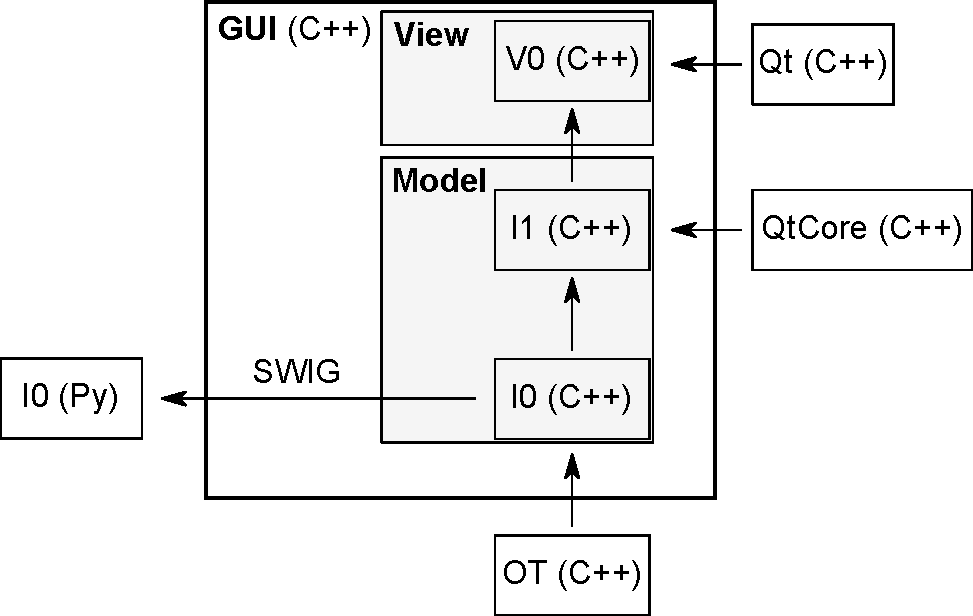
\includegraphics[width=0.95\textwidth]{figures/ArchiGUI-Internal.pdf}
\end{center}

	\end{columns}

\begin{center}
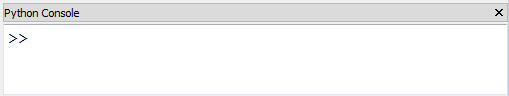
\includegraphics[width=0.9\textwidth]{figures/image007.png}
\end{center}

\end{frame}

%%%%%%%%%%%%%%%%%%%%%%%%%%%%%%%%%%%%%%%%%%%%%%%%%%%%%%%%%%%%%%%%%%%%%%%%%%%%%
\section{Demo backup}

%%%%%%%%%%%%%%%%%%%%%%%%%%%%%%%%%%%%%%%%%%%%%%%%%%%%%%%%%%%%%%%%%%%%%%%%%%%%%

\begin{frame}
\frametitle{Symbolic physical model}

\begin{center}
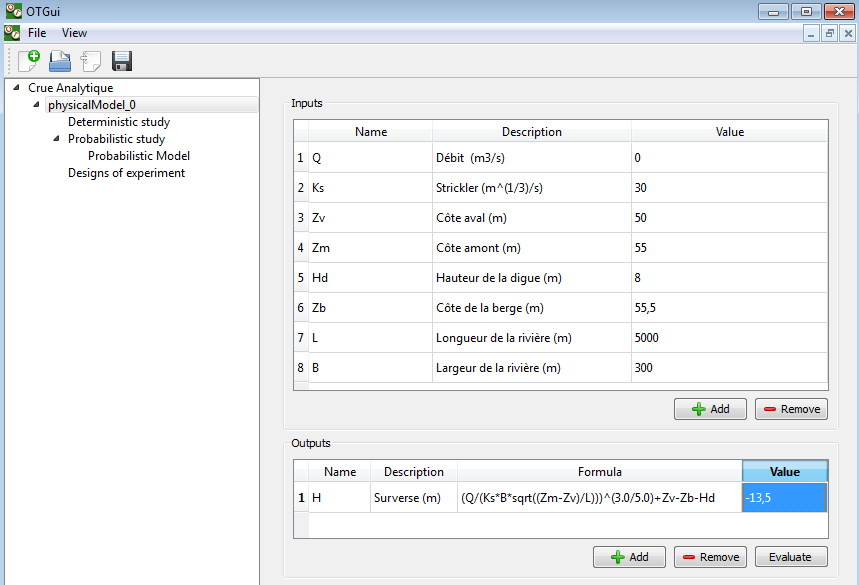
\includegraphics[width=0.9\textwidth]{figures/image009.png}
\end{center}

\end{frame}

%%%%%%%%%%%%%%%%%%%%%%%%%%%%%%%%%%%%%%%%%%%%%%%%%%%%%%%%%%%%%%%%%%%%%%%%%%%%%

\begin{frame}
\frametitle{Probabilistic model}

\begin{center}
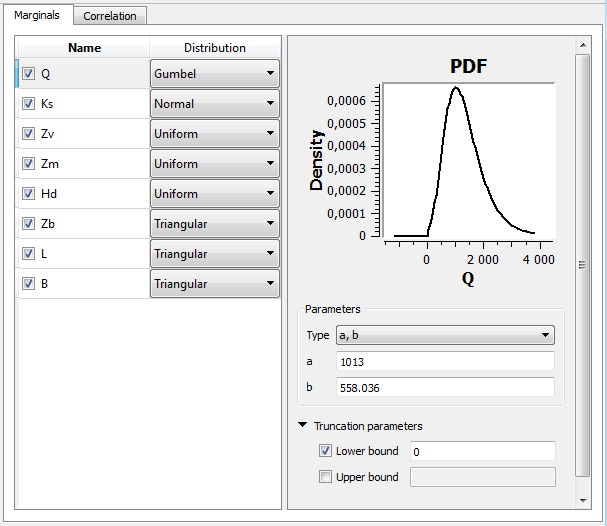
\includegraphics[height=0.8\textheight]{figures/image013.png}
\end{center}

\end{frame}

%%%%%%%%%%%%%%%%%%%%%%%%%%%%%%%%%%%%%%%%%%%%%%%%%%%%%%%%%%%%%%%%%%%%%%%%%%%%%

\begin{frame}
\frametitle{Limit state study : definition of the threshold}

\begin{center}
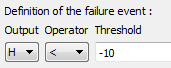
\includegraphics[width=0.4\textwidth]{figures/image015.png}
\end{center}

\end{frame}

%%%%%%%%%%%%%%%%%%%%%%%%%%%%%%%%%%%%%%%%%%%%%%%%%%%%%%%%%%%%%%%%%%%%%%%%%%%%%

\begin{frame}
\frametitle{Limit state study : algorithm parameters}

\begin{center}
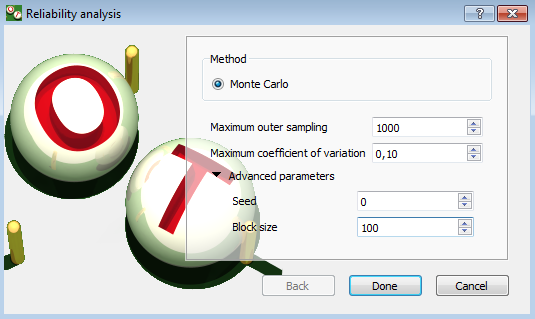
\includegraphics[width=0.95\textwidth]{figures/image017.png}
\end{center}

\end{frame}

%%%%%%%%%%%%%%%%%%%%%%%%%%%%%%%%%%%%%%%%%%%%%%%%%%%%%%%%%%%%%%%%%%%%%%%%%%%%%

\begin{frame}
\frametitle{Limit state study : summary}

\begin{center}
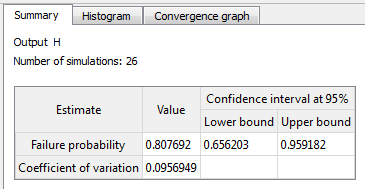
\includegraphics[width=0.7\textwidth]{figures/image019.png}
\end{center}

\end{frame}

%%%%%%%%%%%%%%%%%%%%%%%%%%%%%%%%%%%%%%%%%%%%%%%%%%%%%%%%%%%%%%%%%%%%%%%%%%%%%

\begin{frame}
\frametitle{Limit state study : histogram}

\begin{center}
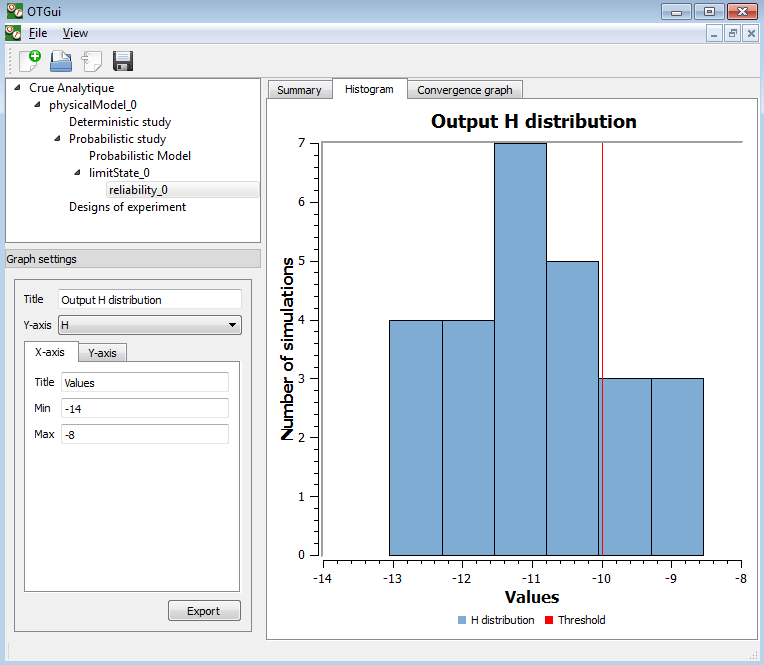
\includegraphics[width=0.7\textwidth]{figures/image021.png}
\end{center}

\end{frame}

%%%%%%%%%%%%%%%%%%%%%%%%%%%%%%%%%%%%%%%%%%%%%%%%%%%%%%%%%%%%%%%%%%%%%%%%%%%%%

\begin{frame}
\frametitle{Central tendency : algorithm parameters}

\begin{center}
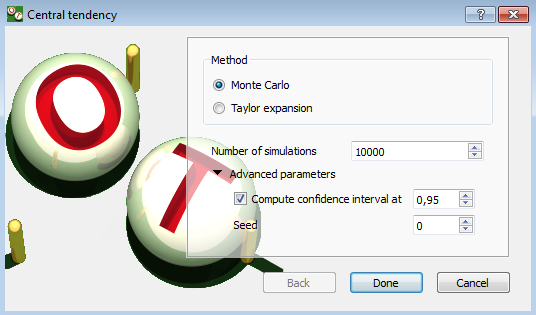
\includegraphics[width=0.8\textwidth]{figures/image023.png}
\end{center}

\end{frame}

%%%%%%%%%%%%%%%%%%%%%%%%%%%%%%%%%%%%%%%%%%%%%%%%%%%%%%%%%%%%%%%%%%%%%%%%%%%%%

\begin{frame}
\frametitle{Central tendency : summary results}

\begin{center}
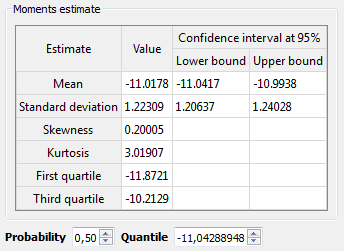
\includegraphics[width=0.8\textwidth]{figures/image025-bottom.png}
\end{center}

\end{frame}

%%%%%%%%%%%%%%%%%%%%%%%%%%%%%%%%%%%%%%%%%%%%%%%%%%%%%%%%%%%%%%%%%%%%%%%%%%%%%

\begin{frame}
\frametitle{Central tendency : summary results}

\begin{center}
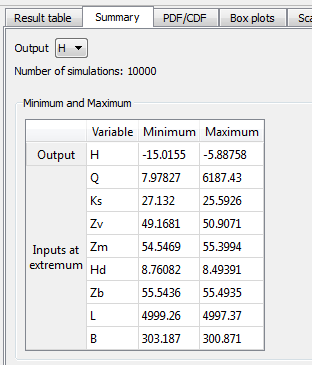
\includegraphics[height=0.8\textheight]{figures/image025-top.png}
\end{center}

\end{frame}

%%%%%%%%%%%%%%%%%%%%%%%%%%%%%%%%%%%%%%%%%%%%%%%%%%%%%%%%%%%%%%%%%%%%%%%%%%%%%

\begin{frame}
\frametitle{Central tendency : scatter plots}

\begin{center}
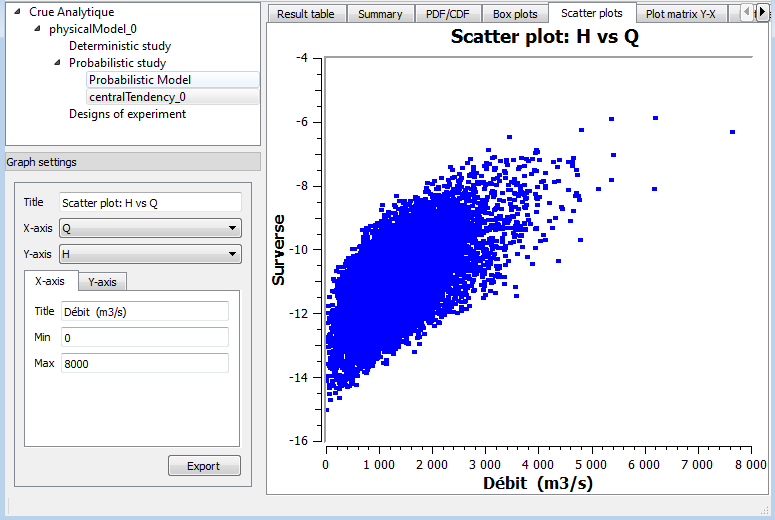
\includegraphics[width=0.8\textwidth]{figures/image028.png}
\end{center}

\end{frame}


%%%%%%%%%%%%%%%%%%%%%%%%%%%%%%%%%%%%%%%%%%%%%%%%%%%%%%%%%%%%%%%%%%%%%%%%%%%%%

\begin{frame}
\frametitle{Sensitivity analysis : Sobol' indices}

\begin{center}
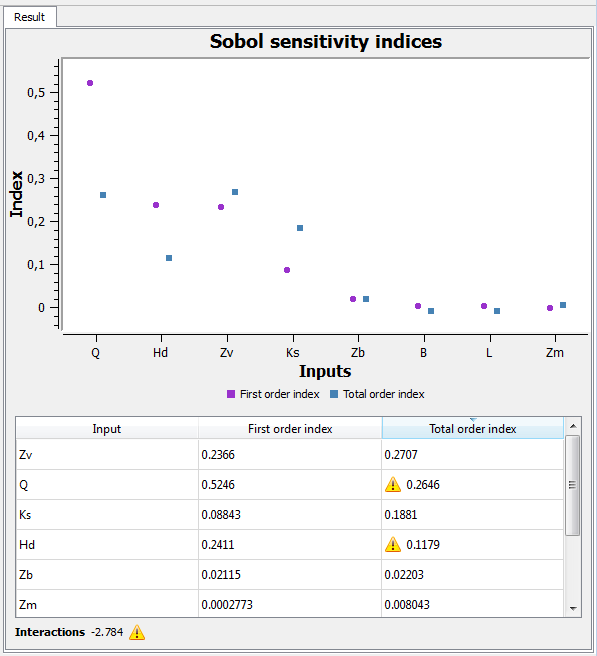
\includegraphics[height=0.8\textheight]{figures/image030.png}
\end{center}

\end{frame}

\end{document}
